%% Преамбула TeX-файла

% 1. Стиль и язык
\documentclass[utf8x, 14pt]{G7-32} % Стиль (по умолчанию будет 14pt)

\usepackage{totcount}

\newtotcounter{citnum} %From the package documentation
\def\oldbibitem{} \let\oldbibitem=\bibitem
\def\bibitem{\stepcounter{citnum}\oldbibitem}

\usepackage{etoolbox}

\newcounter{totfigures}

\providecommand\totfig{}

\makeatletter
\AtEndDocument{%
  \addtocounter{totfigures}{\value{figure}}%
  \immediate\write\@mainaux{%
    \string\gdef\string\totfig{\number\value{totfigures}}%
  }%
}
\makeatother

\pretocmd{\chapter}{\addtocounter{totfigures}{\value{figure}}\setcounter{figure}{0}}{}{}


% Остальные стандартные настройки убраны в preamble.inc.tex.
\sloppy

% Настройки стиля ГОСТ 7-32
% Для начала определяем, хотим мы или нет, чтобы рисунки и таблицы нумеровались в пределах раздела, или нам нужна сквозная нумерация.
\EqInChapter % формулы будут нумероваться в пределах раздела
\TableInChapter % таблицы будут нумероваться в пределах раздела
\PicInChapter % рисунки будут нумероваться в пределах раздела

% Добавляем гипертекстовое оглавление в PDF
\usepackage[
bookmarks=true, colorlinks=true, unicode=true,
urlcolor=black,linkcolor=black, anchorcolor=black,
citecolor=black, menucolor=black, filecolor=black,
]{hyperref}

% Изменение начертания шрифта --- после чего выглядит таймсоподобно.
% apt-get install scalable-cyrfonts-tex

\IfFileExists{cyrtimes.sty}
    {
        \usepackage{cyrtimespatched}
    }
    {
        % А если Times нету, то будет CM...
    }

\usepackage{graphicx}   % Пакет для включения рисунков
\DeclareGraphicsExtensions{.jpg,.pdf,.png}
% С такими оно полями оно работает по-умолчанию:
% \RequirePackage[left=20mm,right=10mm,top=20mm,bottom=20mm,headsep=0pt]{geometry}
% Если вас тошнит от поля в 10мм --- увеличивайте до 20-ти, ну и про переплёт не забывайте:
\geometry{right=20mm}
\geometry{left=30mm}



% Произвольная нумерация списков.
\usepackage{enumerate}
\usepackage{enumitem}
\usepackage{amsmath}
\usepackage{float}
\usepackage{subcaption}
\usepackage{listings}
\usepackage{lastpage}
\pagestyle{myheadings}
\DeclareMathOperator*{\argmax}{arg\,max}
\DeclareMathOperator*{\argmin}{arg\,min}

\setcounter{tocdepth}{1} %Подробность оглавления
%4 это chapter, section, subsection, subsubsection и paragraph
%3 это chapter, section, subsection и subsubsection
%2 это chapter, section, и subsection
%1 это chapter и section
%0 это chapter.


\begin{document}

\frontmatter % выключает нумерацию ВСЕГО; здесь начинаются ненумерованные главы: реферат, введение, глоссарий, сокращения и прочее.
\begin{center}
РЕФЕРАТ
\end{center}

% \large Московский авиационный институт\\[5.5cm]

% \huge Реферат \\[0.6cm] % название работы, затем отступ 0,6см
% \large на тему:  <<Метод идентификации музыкальных
% произведений по аудио фрагментам концертных исполнений>>\\[3.7cm]


% \end{center}

% \begin{flushright}
% Выполнил: студент гр. М8О-406Б \\
% Давид Гринберг \\
% \end{flushright}


% \vfill

% \begin{center}
% \large Москва 2020
% \end{center}

% \thispagestyle{empty}
Выпускная квалификационная работа содержит \pageref{LastPage} страниц, \totfig{}
рисунков, \total{citnum}\ использованных источников.

КОНТЕЙНЕРИЗАЦИЯ, БАЗЫ ДАННЫХ, БРОКЕРЫ СООБЩЕНИЙ, ПАРСИНГ САЙТОВ, ИНТЕРНЕТ
СЕРВЕР, API, СИСТЕМА ШАБЛОНОВ ДЛЯ ДОСТАВКИ HTML СТРАНИЦ, UWSGI, NGINX, ELASTIC
SEARCH, KAFKA, PYTHON.

Выпускная квалификационная работа посвящена поиску оптимальных с точки зрения
масштабирования и эксплуатации компонентов системы, их коммуникации и дальнейшей
виртуализации с целью поиска алгоритмов по имени на интернет ресурсах без
использования официального API.

В теоретической части рассматриваются принципы по которым должна строится
система, описываются выбранные компоненты и их структура. Также производится
сравнение с другими аналогичными продуктами и обосновывается сделанный выбор.

В практической части рассматриваются достигнутая архитектура, методы
отслеживания работы. Кроме того демонстрируется работа системы в целом и каким
способом ее можно маштабировать.


\thispagestyle{empty}
\setcounter{page}{0}
\setcounter{tocdepth}{2}
\setcounter{secnumdepth}{2}
\tableofcontents
\clearpage


\Introduction

Выпускная квалификационная работа посвящена поиску оптимальных с точки зрения
масштабирования и эксплуатации компонентов системы, их коммуникации и дальнейшей
виртуализации с целью поиска алгоритмов по имени на интернет ресурсах без
использования официального API. Объектом исследования является поиск и настройка
оптимального архитектурного решения, которое подходит не только под современные
требования, но и хорошо укладывается в общую концепцию цели ВКР.

Технологии достаточно плотно проникли в образ жизни среднестатистического
человека. Быстро развиваясь, не каждый способен уследить весь прогресс, который
поддерживает нас ежедневно. Почти у каждого есть ЭВМ которая помещается в
карман, или даже надевается на руку. Это все значительно упрощает жизнь в том
плане, что человеку больше не нужно отправлять почтовых голубей и решать
проблемы с ними связанными. Или же, теперь не нужно ждать пока друг вернется
домой и наконец-то возьмет городской телефон. В текущее время, ты можешь быть
всегда на связи, принимать самые оперативные решения и максимально свободен в
доступе к информации.

Но есть одно но. Удобство технологий и простота их использования достается не
бесплатно. Каждый новый программный продукт является потенциальным "кирпичиком"
для следующих разработок. Данный "кирпичик" необходимо поддерживать: производить
обновления безопасности, внедрять новый актуальный функционал (например, если
программа работает с видеофайлами, то внедрять новые кодеки).

В 21 веке мы пользуемся такими программами, о которых в 20 веке и не подумали
бы. Все это, более чем напрямую затрагивает и самих программистов. Когда-то люди
использовали перфокарты, сейчас - специальные среды разработки с подсветкой
синтаксиса, автодополнением, линкером и copilot для разработки на
высокоуровневом языке программирования.

Одной из недостающих утилит для современного разработчика является возможность
быстрого поиска алгоритмов. Обычно эта задача решается "в лоб": пытаемся найти в
интернете аналогичную задачу; открываем книжку по алгоритмам и структурам данным
и пытаемся найти что-то аналогичное и т.п.

Целью данной работы является разработка программного обеспечения для быстрого
развертывания инфраструктуры по поиску алгоритмов на интернет ресурсах,
находимых в общем доступе. Такое ПО будет не только находить алгоритмы, но и
предоставлять возможность по управлению сохраняемыми данными.



\mainmatter

\Main
\hspace{0pt}
\vfill
\begin{center}
ОСНОВНАЯ ЧАСТЬ
\end{center}
\vfill
\hspace{0pt}
\pagebreak

\chapter{Теоретическая часть}
\label{cha:ch_1}

\section{Постановка задачи}
В рамках данной выпускной квалификационной работы предполагается выбрать
компоненты для реализации и разработать инфраструктуру по поиску алгоритмов.

Инфраструктуру в целом требуется разработать в соответствии концепции
микросервисной архитектуры. Плюсом такой реализации является легкая заменяемость
модулей. Также необходимо средство контейнеризации и оркестрации контейнеров.
Необходимо для более легкого развертывания приложений на облачных структурах
(вычислительных серверах).

Логика инфраструктуры будет заключаться в следующем:
\begin{enumerate}[label=\arabic*.]
    \item Считать запрос пользователя. Т.е. предложить ему выбор вписать желаемое самому или выбрать из списка доступных опций;
    \item Произвести поиск по ключевым словам на необходимых интернет ресурсах;
    \item Выделить из возвращенных html страниц необходимые данные (произвести уточняющие запросы, либо запросы перехода на следующую страницу пагинации, если требуется);
    \item Полученные данные положить в базу данных;
    \item Пользователь теперь имеет возможность посмотреть, что нашлось.
\end{enumerate}

\section{Микросервисная архитектура}
Для разработки приложения для данной выпускной квалификационной работы была выбрана микросервисная архитектура.
% https://ru.wikipedia.org/wiki/%D0%9C%D0%B8%D0%BA%D1%80%D0%BE%D1%81%D0%B5%D1%80%D0%B2%D0%B8%D1%81%D0%BD%D0%B0%D1%8F_%D0%B0%D1%80%D1%85%D0%B8%D1%82%D0%B5%D0%BA%D1%82%D1%83%D1%80%D0%B0
Микросервисная архитектура - такой вариант сервис-ориентированной архитектуры
программного обеспечения, который направлен на взаимодействие наиболее
раздробленных, небольших, слабосвязанных и легко модифицируемых модулей, которые
называются микросервисами.

У данной архитектуры есть ряд преимуществ и недостатков. Начнем с преимуществ:
\begin{itemize}
    \item модули (из которых состоит инфраструктура) легко заменяемые (не нужно
        полностью пересобирать и развертывать всю инфраструктуру, при внесении
        небольших изменений);
    \item сервисы могут быть реализованны с помощью разных средств, где
        последние выбираются в пользу высокой эффективности;
    \item архитектура получается симметричная, а не иерархическая.
\end{itemize}

Нельзя обойтись и без недостатков:
\begin{itemize}
    \item Сложность начальной разработки;
    \item Могут возникать сетевые издержки;
    \item Формат сообщений между сервисами должен быть стандартизован, что
        приводит к дополнительным издержкам на поддержание инфраструктуры.
\end{itemize}

% «Создание микросервисов», Сэм Ньюмен, стр 23
Микросервисная архитектура также хорошо отвечает принципу единственной
обязанности -- Single Rsponsibility Principle, которое гласит: «Собирайте вместе
все, что изменяется по одной и той же причине и разделяйте все, что изменяется
по разным причинам».

% https://mcs.mail.ru/blog/prostym-jazykom-o-mikroservisnoj-arhitekture
Для сравнения, в монолитной архитектуре все компоненты соеденены в единое целое.
Вся логика по обработке запросов помещается внутрь одного процесса. Разумеется,
монолиты могут иметь модульную стркутуру -- содержать отдельные классы, функции.
Но связи между этими модулями настолько сильны, что изменение каждого из них
неизбежно отражается на работе приложения в целом.
\begin{figure}[H]
    \centering
    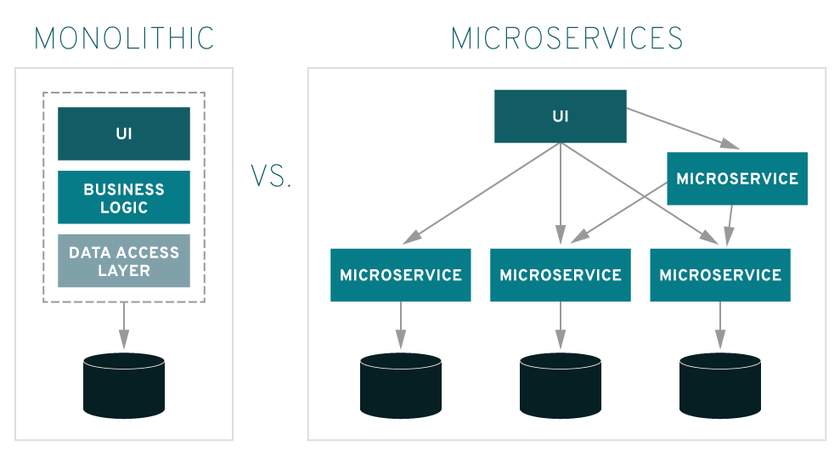
\includegraphics[scale=0.6]{inc/img/Monolithic-vs-microservices.png}
    \caption{Сравнение микросервисной и монолитной архитектуры}
\end{figure}

\section{Технология контейнеризации}
% https://ru.wikipedia.org/wiki/%D0%92%D0%B8%D1%80%D1%82%D1%83%D0%B0%D0%BB%D0%B8%D0%B7%D0%B0%D1%86%D0%B8%D1%8F
По определению виртуализация -- это предоставление набора вычислительных
ресурсов или их логического объединения, абстрагированное от аппаратной
реализации, и обеспечивающее при этом логическую изоляцию друг от друга
вычислительных процессов, выполняемых на одном физическом ресурсе.

% https://habr.com/ru/company/southbridge/blog/530226/
% https://eternalhost.net/blog/razrabotka/docker-kubernetes
Одной из отличительных черт контейнеров от виртуальных машин -- то, что первые
используют возможность не железа, а операционной системы, так называемое
пространство имен. Можно произвести грубое сравнение виртуальных машин и
контейнеров:
% learning docker
\begin{table}[H]
    \centering
    \begin{tabular}{|l|l|}
        \hline
        {\bf Виртуальные машины}                   & {\bf Контейнеры} \\\hline
        Аппаратная виртуализация                   & Виртуализация на уровне ОС \\\hline
        Тяжеловесные                               & Легковесные \\\hline
        Полностью изолированные (более безопасные) & Изолирование на уровне процессов \\\hline
    \end{tabular}
    \caption{Сравнение виртуальных машин и контейнеров}
\end{table}
\begin{figure}[H]
    \centering
    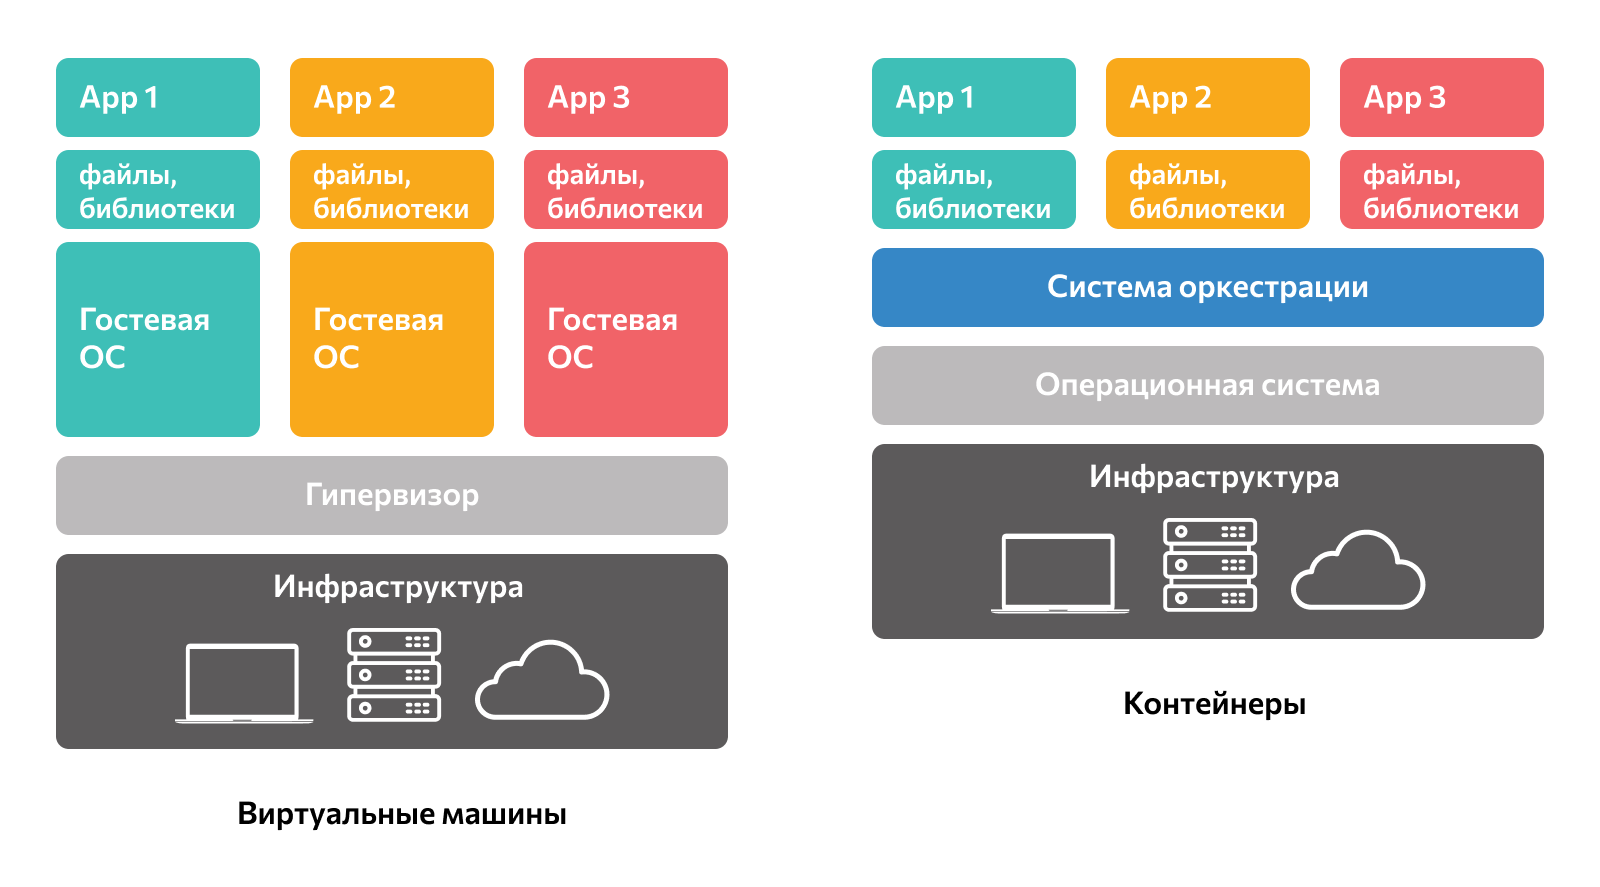
\includegraphics[scale=0.25]{inc/img/cont-vs-virt.png}
    \caption{Сравнение виртуальных машин и контейнеров}
\end{figure}

% https://blog.skillfactory.ru/glossary/kontejnerizacziya/
Технологии контейнеризации решают проблему изолированного запуска приложений и
рабочих сред вне зависимости от системы (должно быть то же ядро) и ПО,
установленных на конкретной машине. Также данная технология позволяет легко
управлять сложными приложениями и средами (упаковывать зависимости, перемещать
решение с системы на систему). 

% TODO: сравнение технологий контейнеризации
\section{Поиск по web-ресурсам}
Для поиска по web-ресурсам безусловно достаточно только возможность совершать
HTTP-запросы (с необходимыми заголовками, сертификатами и т.д.) и читать то, что
сервер возвращает клиенту. Но в целях данной выпускной квалификационной работы
присутствует задача выбрать хорошую архитектуру. Поэтому нужно рассмотреть
фреймворки (или системы), которые позволяют упростить эту самую работу.

% https://pythobyte.com/10-tips-to-avoid-getting-blocked-while-scraping-websites-ncf-bee5b81c/
Также многие сайты стараются скрыть свою информацию от web-ботов. Возможно это
обусловленно тем, что последние злоупотребляют общедоступной информацией либо
вычислительной мощностью, которую сервер выделяет на пользователя. Поэтому, на
таких серверах могут быть настроенны политики запрета доступа к контенту при
слишком частом запросе страницы.

% https://coderlessons.com/tutorials/devops/uchitsia-scrapy/scrapy-kratkoe-rukovodstvo
Свойства которыми должен обладать фреймворк при работе с web-ресурсами:
\begin{itemize}
    \item Быть масштабируемым на большие проекты сканирования;
    \item Асинхронная обработка запросов;
    % TODO: сделать сноску на селекторы
    \item Встроенный механизм работы с селекторами;
    % TODO: сделать сноску на дросселирование
    \item Обладает механизмом автоматического дросселирования;
    \item Генерация результатов в разных структурных текстовых форматах.
\end{itemize}

% сравнение requests, beautiful soup 4, lxml, selenium, scrapy

Фреймворк на python -- scrapy удовлетворяет всем вышеперечисленным свойствам.
Более того для него написанна серверная часть scrapyd, которая позволяет
размещать "пауков" на мощных серверах, с последующим запуском либо по
расписанию, либо по http-запросу.
\begin{figure}[H]
    \centering
    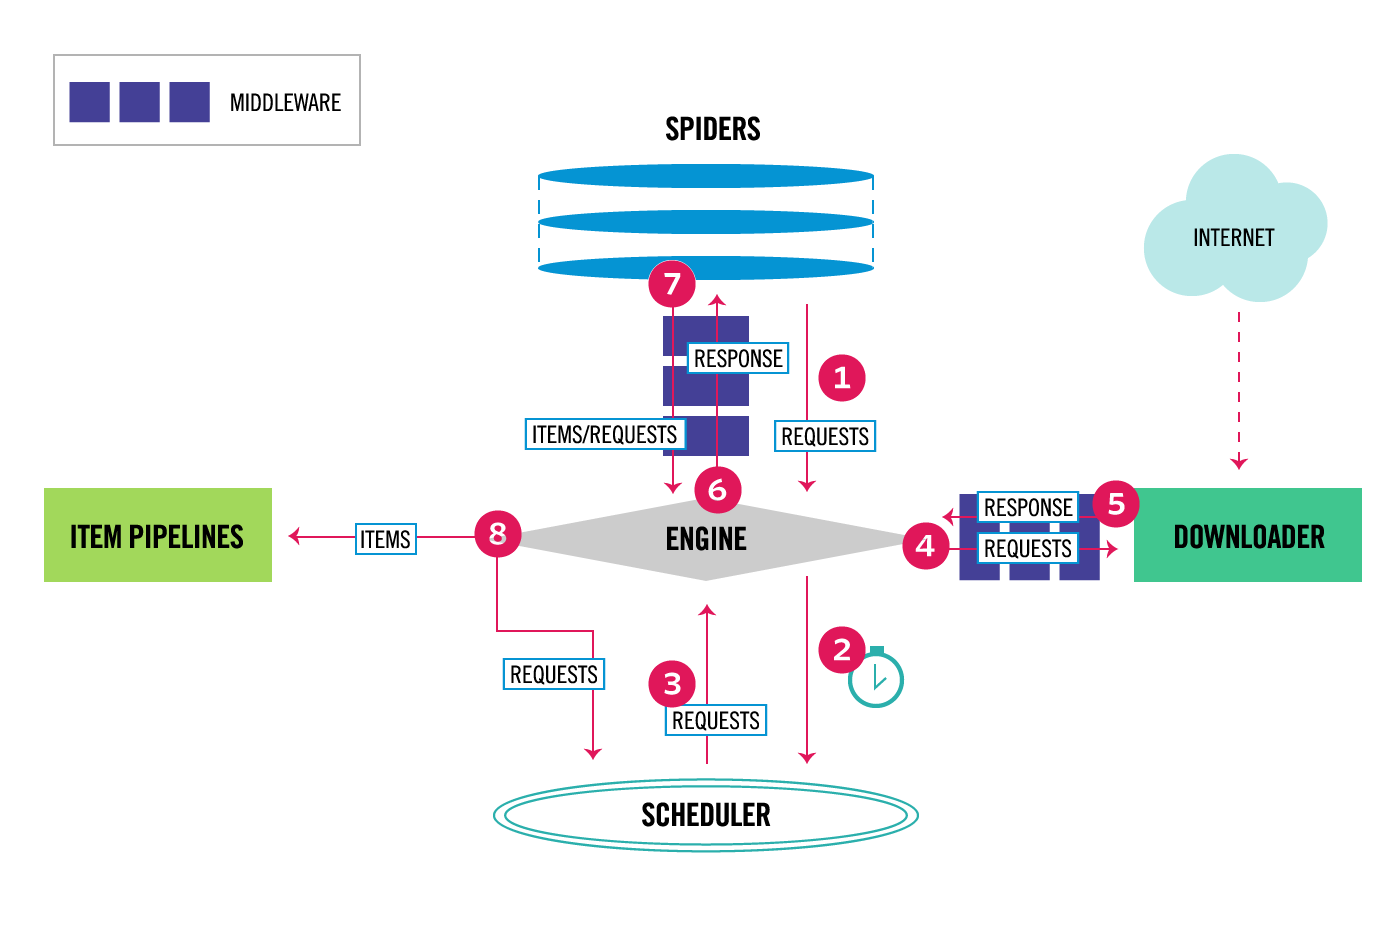
\includegraphics[scale=0.35]{inc/img/scrapy_architecture.png}
    \caption{Архитектура scrapy}
\end{figure}

% TODO: сделать сноску что этот файл обозначает
Также в этом модуле можно настроить много других политик доступа к интернет ресурсам. В такие политики входят:
\begin{itemize}
    \item Чтение файла \verb|robots.txt|;
    \item Лист прокси;
    \item Ротация заголвков и куков.
\end{itemize}

Данная библиотека позволяет полностью посмотреть список настроек, добавить свои,
и написать такую конфигурацию системы, чтобы не добавить свою вычислительную
сеть в черный список целевой структуры.

\section{Серверная часть}
% кто-то читает порт и является в то же время прокси: nginx
% uwsgi: передает сообщения на python
% flask: построен на основе uwsgi для того чтобы просто принимать сообщения, а
% сам является обработчиком

\section{Брокер сообщений}
\section{База данных}


\chapter{Практическая часть}
\label{cha:ch_2}

\section{Проектирование архитектуры}
% Какая задача поставлена
На основе данной задачи выделяются следующие подзадачи, которые необходимо
выполнить, для успешной реализации инфраструктуры:
\begin{enumerate}[label=\arabic*.]
    \item Описать возможные процессы взаимодействия между компонентами системы.
        Удобно произвести описание с помощью Use-Case диаграммы;
    \item Смоделировать архитектуру приложения: какие компоненты будут
        взаимодействовать друг с другом;
    \item Далее равнозначные задачи, которые не обязательно выполнять
        последовательно: написать файлы запуска и написать кодовую базу для
        запуска каждой из компоненты системы.
\end{enumerate}

Далее рассмотрим каждый из пунктов подробнее, опишем способ реализации,
возникшие проблемы и пути решения.

\section{Use-Case диаграмма}
\section{Архитектура приложения}
\section{Разработка практических решений}
\subsection{Docker}
\subsection{Docker Compose}
\subsection{Scrapy}
\subsection{Scrapyd}
\subsection{Flask}
\subsection{Kafka}
\subsection{Zookeeper}
\subsection{Kafka Connect}
\subsection{Elastic Search}


\backmatter %% Здесь заканчивается нумерованная часть документа и начинаются ссылки и
            %% заключение

\Conclusion % заключение к отчёту

При выполнении ВКР были решены следующие задачи:
\begin{enumerate}[label=\arabic*.]
    \item Спроектирована микросервисная архитектура;
    \item Выбраны модули для реализации;
    \item Все сервисы были развернуты с участием в конечной инфрастуктуре;
\end{enumerate}

Даннная инфраструктура позволяет клиентам искать алгоритмы по имени, а затем
сохранять их в базу данных. Администраторы могут проследить работу всех
компонентов.

Также возможно настроить распределение узлов хранения и передачи сообщений. Так
как все сервисы контейнезированы, это дало несколько преимуществ:
\begin{enumerate}[label=\arabic*.]
    \item Все зависимости будут скомпанованы с самим сервисов;
    \item Результат выполнения более предсказуем (в сравнении с обычной
        установкой сервиса на другую машину);
    \item Легкая модификация конфигурационных файлов;
    \item В отличие от виртуализации на уровне операционной системы,
        контейнеры более легкие.
\end{enumerate}

% Очень интересно было во всем этом разобраться и почитать углубленно, т.к.
% планирую работать в это отрасли, да и вообще, очень захватывает написание
% больших распределенных систем, которые должны работать как по часам. И возникает
% хорошее чувство, когда при долгом написании отдельных компонентов, все это
% складывается воедино -- в одну целую компоненту.



\nocite{*}
\bibliographystyle{gost780u}
\begin{thebibliography}{9}
    \bibitem{tsai} Tsai, T. (2016). Audio Hashprints: Theory \& Application.
    (Doctoral dissertation, EECS Department, University of California, Berkeley).

    \bibitem{chromaprint}
    Yan Ke, Derek Hoiem, Rahul Sukthankar. (2005). Computer Vision for Music
    Identification, Proceedings of Computer Vision and Pattern Recognition.

    \bibitem{hnsw} Leonid Boytsov and Bilegsaikhan Naidan (2013).
    Engineering Efficient and Effective Non-metric Space Library.
    In Similarity Search and Applications - 6th International Conference, SISAP 2013,
    A Coru\~na, Spain, October 2-4, 2013, Proceedings (pp. 280–293). Springer.

    \bibitem{essentia} Bogdanov, D., Wack N., Gómez E., Gulati S., Herrera P., Mayor O., et al. (2013).
    ESSENTIA: an Audio Analysis Library for Music Information Retrieval. International Society for Music Information Retrieval Conference (ISMIR'13). 493-498.

    \bibitem{cqt} Schörkhuber, C., Klapuri, A., Holighaus, N., \& Dörfler, M. (n.d.).
    A Matlab Toolbox for Efficient Perfect Reconstruction Time-Frequency Transforms with Log-Frequency
    Resolution

    \bibitem{eigen} Gael Guennebaud, Benoit Jacob, \& others. (2010). Eigen v3.

    \bibitem{tf} T. Huang, C. Lin, G. Guo and M. Wong, "Cpp-Taskflow: Fast Task-Based Parallel
    Programming Using Modern C++," 2019 IEEE International Parallel and Distributed Processing
    Symposium (IPDPS), Rio de Janeiro, Brazil, 2019, pp. 974-983, doi: 10.1109/IPDPS.2019.00105.
\end{thebibliography}

\appendix   % Тут идут приложения

% \chapter{Первое Приложение}

\end{document}
